%---------------------------------------------------------------
%---------------------------------------------------------------
\chapter{Erzeugung der Dinge, die nicht von PCA vorgegeben sind}
\label{chapter:non_pca_things}

Ein Punkt im PCA-Raum gibt schon viele Eigenschaften des zu generierenden Skeletts vor. Zu den Dingen, die noch festgelegt werden müssen, zählen \zb die Anzahl und Anordnung der Wirbel und Rippen und vor allem die Ausrichtung der Extremitäten.

\todo{Übeblick über den Ablauf des Algorithmus}

%-----------------------------------------------
\section{Ausrichtung der Extremitäten}
\label{section:extremity_generation}

% Allgemeine Schwierigkeit Extremitäten zu positionieren
Das Skelett soll in einer Art Ruheposition dargestellt werden. Im Allgemeinen ist aber nicht klar wie die Ruheposition einer Extremität aussieht. Das ist schon allein daran zu erkennen, dass auf Darstellungen von Wirbeltierskeletten Flügel manchmal ausgestreckt und manchmal eingefaltet sind. Auch Beine sind meist so angeordnet, dass es aussieht als würde das entprechende Tier gerade laufen. Dies ist auf Abbildung \ref{klippschliefer} am Beispiel des Klippschliefers sehr gut zu sehen.

 \begin{figure}
  \centering
  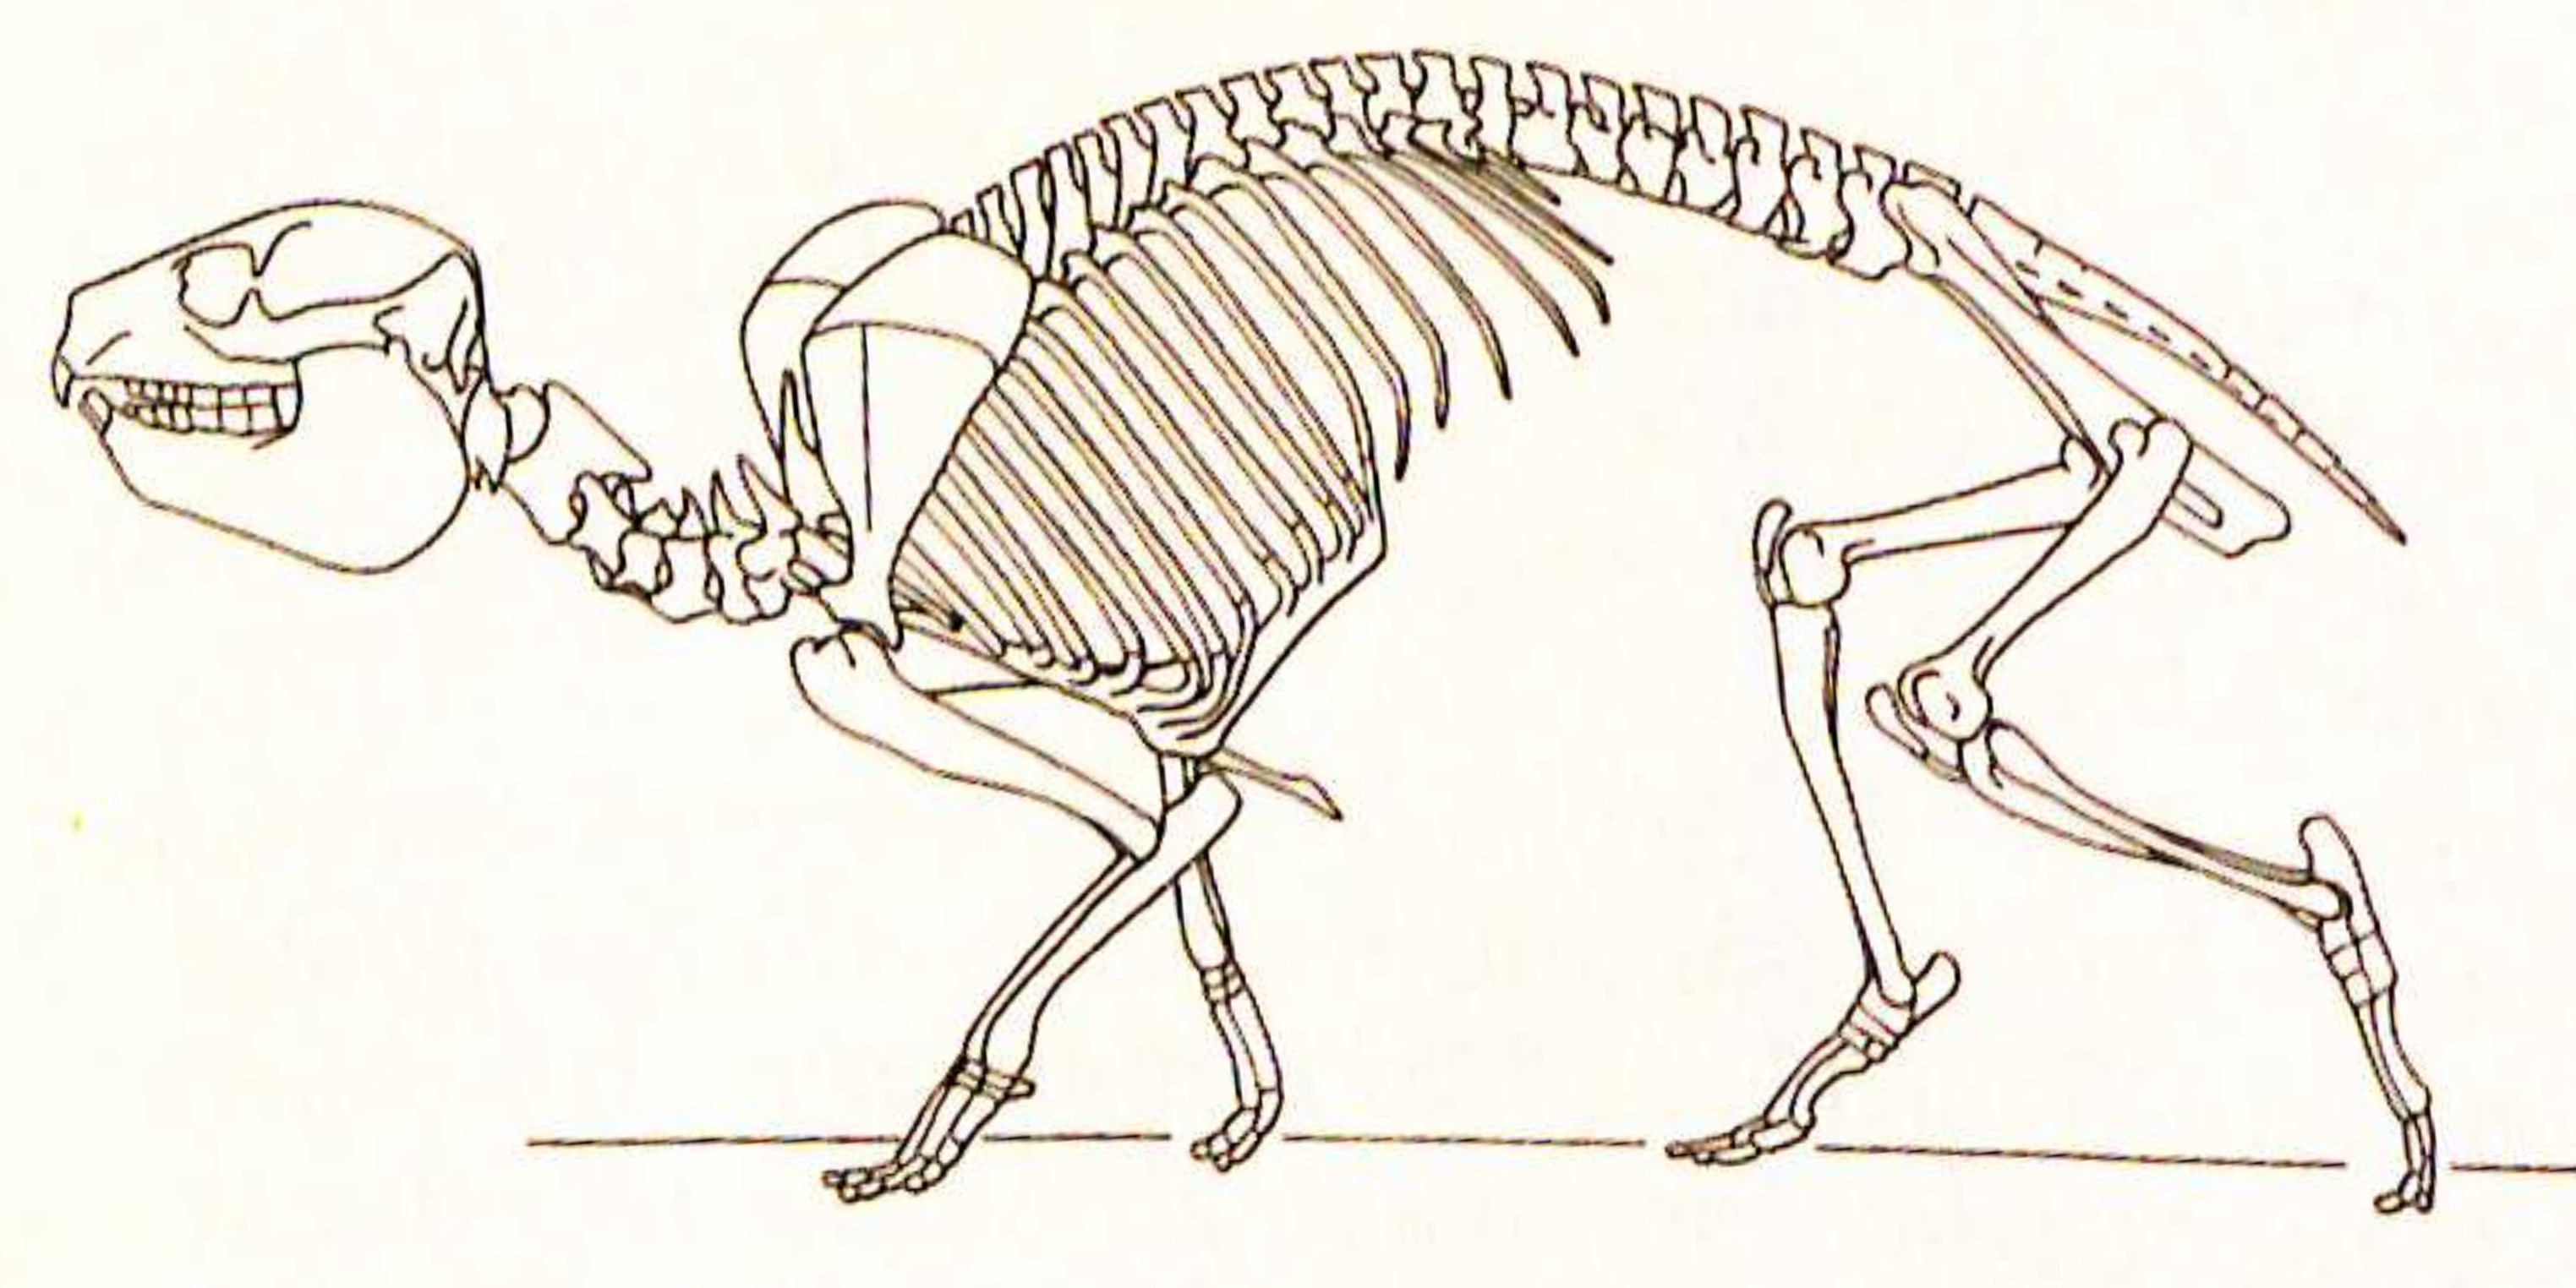
\includegraphics{../PCA/Skelettbilder/Klippschliefer.jpg}
  \caption{Skelett eines Klippschliefers. Dieses Bild wurde auch als Eingabe für die PCA verwendet.}
  \label{klippschliefer}
 \end{figure}

Wie in Kapitel \ref{chapter:pca} zur PCA schon erwähnt, ist es deshalb auch schwer möglich die Ausrichtung der Extremitäten \bzw die Winkel an den Gelenken als zusätzliche Dimension in den PCA-Raum mitaufzunehmen.

Die Positionierung der Extremitäten bleibt also ein Problem mit unklaren Anforderungen und vielen Freitheitsgraden.

% Einteilung in Kategorien
Ein erster Schritt an das Problem heranzugehen, ist es in kleinere Unterprobleme zu zerteilen.
Extremitäten können anhand ihrer Funktion in vier Kategorien eingeteilt werden:
Flügel, Flossen, Extremitäten mit Bodenkontakt (im Folgenden als Beine bezeichnet), und Extremitäten ohne Bodenkontakt (im Folgenden als Arme bezeichnet).

Für Flügel, Flossen und Arme gibt es keine besonderen Anforderungen außer, dass sie als solche zu erkennen sein sollten. Deshalb werden sie nach folgenden simplen Anweisungen orientiert:
\todo{Beispielbilder?}
\begin{itemize}
 \item Flossen: Ausrichtung gerade nach hinten (orientiert an Welt-x-Achse)
 \item Arme: Der Oberarm zeigt senkrecht nach unten (orientiert an Welt-y-Achse), im Ellenbogengelenk ist ein $90^{\circ}$ Winkel und die Hand verlängert Unterarm nach vorne.
 \item Flügel: Jedes beteiligte Gelenk hat ein Intervall mit festen Grenzen speziell für Flügel, aus dem zufällig ein Winkel gewählt wird.
\end{itemize}

Nun bleibt nur doch die Ausrichtung der Beine, für die die zusätzliche Anforderung gilt, dass sie den Boden berühren sollen.


%- - - - - - - - - - - - - - - - - - 
\subsection{Berechnung der Bodenhöhe}
\label{floor_height}

% Warum nicht Höhe 0?
Zunächst könnte man davon ausgehen, dass der Boden einfach auf Höhe null sein sollte. Das Problem hierbei ist aber, dass die von der PCA berechneten Längen für die Extremitäten meist so kurz sind, dass die Beine dann den Boden nicht mehr erreichen würden. Das liegt daran, dass auf den Bildern, die als Eingabebeispiele für die PCA verwendet wurden, der Boden meistens nicht ganz am unteren Rand ist. Hier würde rigoroses Abschneiden der Bilder auf Fußhöhe wahrscheinlich helfen, es würde in vielen Fällen aber auch ein Großteil der Füße verloren gehen.

% Berechnung
Die Höhe des Bodens wird also anhand der von der PCA generierten Längen der Extremitäten festgelegt.
Theoretisch würde es reichen einfach das kürzeste Bein im komplett ausgestreckten Zustand zu betrachten und den Boden auf die Höhe dessen Endpunkts festzulegen.
Das führt aber zu unnatürlich aussehenden Beinen, da das kürzeste Bein dann genau senkrecht nach unten führen muss um den Boden zu erreichen.

Deshalb wird nur ein bestimmter Anteil der Länge der Beine betrachtet. So wird erzwungen, dass die Beine, wenn sie auf dem neu definierten Boden stehen, auch etwas gekrümmt sind. \todo{Variation der bent ratio?}

Wie in Kapitel \ref{chapter:biology} beschreiben gibt es verschiedene Arten von Füßen. Die oben beschriebene Berechnung geht davon aus, dass der Boden mit der Fußspitze berührt wird. Aber natürlich gibt es auch Wirbeltiere, die mit dem flachen Fuß auf der Erde stehen.
Deshalb wird zusätzlich zur Bodenhöhe noch eine Wahrscheinlichkeit berechnet, dass Verse \bzw Handgelenk den Boden berühren.

Wird die Bodenhöhe nach oben verschoben, weil die Beine insgesamt zu kurz sind, ist diese Wahrscheinlichkeit null.
Sind die Beine so lang, dass schon ohne die Bodenhöhe anzupassen die Verse \bzw das Handgelenk auf den Boden reicht, so ist sie eins.
Ansonsten ist die Wahrscheinlichkeit 
\[\frac{\textrm{Beinlänge} - \textrm{Höhe des Extremitätengürtels über $0$}}{\textrm{Länge des Fußes}}\]
Wenn es Vorder- und Hinterbeine gibt, so wird für beide diese Wahrscheinlichkeit berechnet und dann der Mittelwert genommen. Denn es ist sinnvoll, dass alle Beine den gleichen Punkt auf den Boden bringen.
Deshalb legt auch das erste Bein, das generiert wird, basierend auf der oben berechneten Wahrscheinlichkeit, fest, welcher Punkt gewählt wird.


%- - - - - - - - - - - - - - - - - - - - - - - - -
\subsection{Algorithmus zur Ausrichtung der Beine}
\label{leg_algo}

\todo{Absatz über IK, lcp (linear complementary problem) (nicht Hauptaugenmerk / Ziel der Arbeit ist etwas anderes / reicht für Proof of Concept, bei Animationen muss große Maschinerie sowieso nochmal angeworfen werden)}

% \begin{algorithm}
%  \caption{Beinalgorithmus}
%  \label{beinalgo}
%  
%  \begin{algorithmic}
%     \STATE{step = 0\\
%     maxSteps = 50\\
%     angleStepSize = $40^\circ$}
% 
%     \WHILE{floor not reached and step < maxSteps}
%         \FORALL{joints}
%             \IF{child bone of joint has not reached floor and movement nearer to floor possible}
%                 \STATE try change joint angle
%             \ENDIF
%         \ENDFOR
%         \IF{angleStepSize > eps}
%             \STATE reduce angleStepSize
%         \ENDIF
%     \ENDWHILE
%  \end{algorithmic}
% \end{algorithm}
\todo{Pseudocode?}

% iterativ, Drehrichtung
Der hier verwendete Algorithmus zur Ausrichtung der Beine geht iterativ vor.
In jedem Schritt wird für jedes Gelenk berechnet ob sein Winkel vergrößert oder verkleinert werden muss um den dazugehörigen Knochen näher zum Boden zu bewegen.
Mit dem "`dazugehörigen"' Knochen ist hier derjenige der beiden an das Gelenk anschließenden Knochen gemeint, der das Kindelement des anderen ist.
Die Drehrichtung lässt sich relativ leicht herausfinden indem die Ausrichtung des Knochens mit der Welt-y-Achse verglichen wird. Je senkrechter der Knochen ausgerichtet ist, desto ausgestreckter ist das Bein.
\todo{Schaubilder für verschiedene Gelenkarten?}

% Einschränkungen der Gelenke
Zusätzlich gibt es für jedes Gelenk und jeden Freitheitsgrad einen minimalen und einen maximalen Winkel, der eingenommen werden kann. Dieses Intervall hängt von den anatomischen Möglichkeiten des Gelenks ab und von den Winkeln, die in einer "`sinnvollen"' Ruheposition eingenommen werden können. 
\todo{ist das überhaupt eine Einschränkung?}
Es gibt also lokale Einschränkungen je nach Gelenk und globale Randbedingungen. % Problematik mit lokalen Winkelkonstraints vs. globalen Berechnungen für Abstand zum Boden?

% Startposition, Bewegungseinschränkungen
Die Startposition der Extremität ist maximal angewinkelt. Die Gelenke beginnen also mit ihren kleinst- \bzw größtmöglichen Winkeln. In den folgenden Iterationen wird dann derjenige Endpunkt der Extremität dem Boden genähert, der zum Schluss Bodenkontakt haben soll.
Ohne weitere Einschränkungen kann es nun passieren, dass unnatürliche Positionen auftreten, in denen \zb der Fußspann näher am Boden ist als die Fußsohle.
Oder es kann passieren, dass ein Knochen über die positive Welt-y-Achse hinaus gedreht wird. Das Problem dabei ist, dass die Einschränkungen an den Gelenken nicht zulassen, dass der Knochen sich unbegrenzt in diese Richtung weiterdreht und der Knochen dann "`feststeckt"'. Deshalb wird nach jeder Drehung festgestellt ob so eine Situation eingetreten ist und wenn ja, wird die Drehung rückgängig gemacht.
Die Drehung wird ebenfalls rückgängig gemacht, falls sie bewirkt, dass die Knochen unterhalb der Bodenhöhe landen.
\todo{Beispielbilder}
So ist zu jeder Zeit garantiert, dass die Knochen auf der "`richtigen"' Seite der y-Achse liegen und nicht unterhalb der Bodenhöhe sind. % Invarianten

% Verkleinerung der Größe der Drehwinkel
In jeder Iteration werden die Winkel, um den die Gelenke gedreht werden, um einen bestimmten Anteil verkleinert. Zu Beginn soll, mit großen Veränderungen, eine grobe Ausrichtung der Gelenke vorgenommen werden, die dann immer weiter verfeinert wird.
Der Startwinkel darf nicht zu klein sein, weil die Gelenke sonst ihre Zielpositionen nicht erreichen können. Ist der Startwinkel allerdings zu groß, bewirkt es in vielen Fällen nur, dass die Drehung nicht durchgeführt werden kann, weil die oben genannten Randbedingungen verletzt werden.\\
Die Verkleinerung des Winkels darf nicht zu schnell geschehen, weil dann wiederum die Endposition nicht erreicht werden kann. Wenn sie aber zu langsam geschieht passiert in vielen Schritten wiederum nichts wegen verletzter Randbingungen.\\
Durch Ausprobieren wurden folgende Zahlen als sinnvoll erachtet: Startwinkel $40^{\circ}$, später dann jeweils $\frac{6}{7}$ davon.

Falls sich der Abstand zum Boden kaum verändert, liegt also die Vermutung nahe, dass die Gradzahl zu groß ist und deshalb alle möglichen Winkeländerungen invalide sind. Deshalb wird in diesem Fall die Gradzahl für die nächste Iteration stärker verkleinert (halbiert).

\todo{Wkten für Gelenke, Vorteil?}

% Zweiter Freiheitsgrad
Theoretisch haben das Hüft- und das Schultergelenk nicht nur einen, sonder zwei Freiheitsgrade. Der Oberschenkel lässt sich nicht nur nach vorne und hinten bewegen, sondern auch seitlich abspreizen. Das lässt sich auch leicht als zweite Art von Gelenk im Code abbilden. Allerdings liefert der Algorithmus dann oft seltsam anmutende breitbeinige Tiere.
Deshalb wurde der zweite Freiheitsgrad hier außen vor gelassen.
Obwohl es natürlich in der Natur auch viele Tiere mit nach außen gestellten Beinen gibt, wie \zb Echsen.
% + max angewinkelte Pos komisch und Drehrichtung ändert sich je nach anderen Winkel

% Probleme bei sehr kurzen Beinen
Treten sehr kurzen Beinen auf, hat der Algorithmus außerdem einige kleine Probleme. Diese werden genauer in Abschnitt \ref{leg_positioning_short_legs} beschrieben. Da die Beine aber in diesen Fällen, wie gesagt, sehr kurz sind, ist es für den Gesamteindruck gar nicht besonders wichtig wie genau sie angeordnet sind.

% Vergleich echter und generierter Beinstellungen
Wie in Kapitel \ref{chapter:additional_features} beschrieben, lassen sich auch die Eingabebeispiele der PCA laden. Bei ihnen sind dann alle Attribute, die die PCA liefert, schon festgelegt. Alle anderen müssen jedoch noch generiert werden.
Dazu gehören auch die Beine.
Vergleicht man nun die Beinstellung, die der oben beschriebene Algorithmus generiert, mit der Beinstellung auf dem Eingabebild, lassen sich teilweise sehr große Unterschiede feststellen. \todo{gutes und schlechtes Beispiel (schlecht: Brachiosaurus, Elefant)}

% Mehr Infos nötig für Verbesserungen
Um in allen Fällen eine realistisch wirkende Positionierung der Beine zu bekommen, müsste noch sehr viel mehr Arbeit in den Algorithmus gesteckt werden. Außerdem bräuchte der Algorithmus mehr Informationen zum Tier. Solche Zusatzinformationen könnten beispielsweise die Art des Fußes oder die Fortbewegungsart sein. Auch könnte es helfen, wenn es eine sinnvolle Möglichkeit gäbe die Winkel an den Gelenken als Dimension für die PCA mitaufzunehmen. Dafür müsste man sich aber, wie zu Beginn des Kapitels schon erwähnt, auf eine kanonische Ruheposition einigen und dann auch noch Beispiele in genau dieser Position finden.

% für Weiterverwendung werden Beine sowieso angepasst
Ein fertig generiertes Skelett wird höchstwahrscheinlich auch noch "`weiterverarbeitet"'. Soll \zb ein animiertes Tier daraus werden, so müssen Bewegungszyklen geschaffen werden. Dafür muss jedes Gelenk vielfach bewegt werden. Soll ein Tier mit Haut und Muskeln daraus werden, so müssen Muskeln an den Knochen ansetzen, die dann einen nicht unerheblichen Anteil an der Positionierung der Beine haben.

% Beinalgo nicht weiter anpassen
Die von dem hier beschriebenen Algorithmus generierte Position kann also gut als erster Eindruck dienen muss aber in den meisten Fällen noch angepasst werden. Ausgehend von der gegebenen Datenlagen und von den zu erwartenden Anwendungen ist es aber nicht sinnvoll den Algorithmus weiter zu verfeinern.

%--------------------------------------
\section{Zusätzliche Ansatzpunkte für Extremitäten}

Ansatzpunkte für Extremitäten sind natürlich zunächst der Hüftgürtel und der Schultergürtel. Um auch die Generierung fantastischer Tiere zu ermöglichen, ist es aber möglich dies zu erweitern.\\
\todo{andere Möglichkeiten fantastische Tiere zu generieren?}

Eine einfache Möglichkeit ist hier zunächst die Anzahl der möglichen Extremitätenpaare von zwei auf vier zu erhöhen, indem einfach an der Hüfte und der Schulter jeweils zwei Paare ansetzen dürfen. Dafür wurden an der Hüfte \bzw der Schulter mehrere Gelenke direkt hintereinander angelegt, an denen Extremitäten ansetzen können.\\
Flügel und Arme dürfen hierbei weiterhin nur an der Schulter ansetzen, Beine und Flossen an beiden Stellen. Der Grund dafür ist, dass die meisten generierten Skelette seltsam wirken, wenn an der Hüfte Flügel oder Arme ansetzen und dafür an der Schulter Beine beginnen. Das liegt daran, dass existierende Tiere mit Flügeln oder Armen ihren Schwerpunkt im hinteren Bereich haben und sie auf den Hinterbeinen stehen. Deshalb wird die Wirbelsäule durch die PCA auch dementsprechend angelegt.

% mehr Extremitätengürtel auf dem Rücken
Eine Überlegung war auch zwischen Schulter und Hüfte weitere Extremitätengürtel anzubringen. Das stellt sich aber als schwierig heraus. Die Wirbelsäule ist zwischen Hüfte und Schulter nach oben geschwungen und im Bauchraum befinden sich die meisten Organe des Tieres. Ein zusätzlicher Extremitätengürtel würde den Bauchraum einschränken. Außerdem wirkt dann auch die nach oben geschwungene Wirbelsäule anatomisch seltsam.
"`Verdoppelt"' man die Schwingung der Wirbelsäule und hängt einfach einen weiteren Rücken hinten oder vorne an, so wirkt es ebenso seltsam, da dann die "`Höcker"' der Wirbelsäule für das Tier wahrscheinlich nicht wirklich ein Vorteil sind und nur die Fortbewegung erschweren.

% zweiter Schultergürtel
Eine weitere Idee, die auch umgesetzt wurde, ist, eine Art Zentauren zu ermöglichen. Hat das Tier einen Hals, der lang genug ist, kann darauf ein weiterer Schultergürtel kurz unterhalb vom Kopf angebracht werden. An diesem Schultergürtel dürfen dann alle Arten von Extremitäten außer Beinen ansetzen. Das wirkt tatsächlich meist auch anatomisch einigermaßen sinnvoll.

%- - - - - - - - - - - - - - - - - - - 
\subsection{Anordnung der Extremitäten}

\begin{itemize}
 \item wenn Beispiele geladen werden Anzahl und Art der Extremitäten nicht unbedingt richtig (bei PCA Beispiel)
 \item Anzahl der Extremitäten orientiert sich an Benutzereingabe
 \item falls keine Benutzereingabe, dann orientiert es sich an den von der PCA ausgespuckten Wahrscheinlichkeiten für Beine und Flügel
 \item die Position jeder Extremität wird zufällig aus der Menge der möglichen Positionen ausgewählt. Ist für eine Extremität kein Platz mehr, wird geschaut, ob andere Extremität an eine andere Position wechseln kann um Platz zu schaffen
 \item da Positionen nicht deterministisch kommt es bei Tieren mit mehreren möglichen Anordnungen zu unterschiedlichen Ergebnissen bei gleicher Eingabe
 \item da die Anzahl der Arme und Flossen nicht mit PCA erhoben kann sie für die Eingabebeispiele der PCA nicht rekonstruiert werden. Deshalb kann Benutzer hier eigene Angaben machen.
 \item nachdem Extremitäten zugeteilt wurden, werden sie nochmal "`verteilt"', damit nicht \zb zwei Beine an Hüfte aber keins an Schulter \todo{sinnvoll?}
 \item wenn es keine Angabe für die Anzahl der Flügel gibt, werden diese mit der PCA Wkt generiert, aber max ein Paar pro Schultergürtel; bei Beinen wir die Wkt (kann auch 2 sein) auf- oder abgerundet
 \item Arme werden ebenfalls mit Flügelwkt generiert (auch max 1 pro Schultergürtel)
 \item Flossen werden in komplett leere Extremitätengürtel generiert, wenn sie nicht zu lang wären
\end{itemize}


%---------------------------------------------------
\section{Weitere Dinge, die generiert werden müssen}

\begin{itemize}
 \item Wirbel
 \item Rippen (wieviele Rippen, wie lang ist Brustkorb in x-Richtung)
 \item Kopf
 \item Schulter 
\end{itemize}
